\documentclass{beamer}
\usetheme{Amsterdam}

\usepackage[utf8]{inputenc}
\usepackage[style=authoryear,maxcitenames=3,maxnames=3,maxbibnames=100,backend=biber,backref=true,block=none,url=false]{biblatex}
\DeclareLanguageMapping{english}{custom-english-ordinal-sscript}
\DeclareFieldFormat{edition}%
                   {\ifinteger{#1}%
                    {\mkbibordedition{#1}\addthinspace{}ed.}%
                    {#1\isdot}}
\DeclareFieldFormat{journaltitle}{\mkbibemph{#1},} % italic journal title with comma
\DeclareFieldFormat[inbook,thesis]{title}{\mkbibemph{#1}\addperiod} % italic title with period
\DeclareFieldFormat[article,incollection,inproceedings]{title}{#1} % title of journal article is printed as normal text
\addbibresource{bibliography.bib}
\usepackage{tikz}
\usepackage[english]{babel}
\usepackage{upquote}
\usepackage{color}
\usepackage{appendix}
\usepackage{listings}
\usepackage{booktabs}
\usepackage{longtable}
\usepackage{tikz-qtree}
\tikzset{>=latex}
\usetikzlibrary{shapes,arrows,trees}
\def\addsquare#1{\tikz\node[draw]{#1};}
\tikzstyle{block} = [rectangle, draw, text width=5em, text centered, rounded corners, minimum height=4em]
\tikzstyle{line} = [draw, -latex']

\title{Foundations of Language Technology}
\subtitle{Final Project Report}
\author{Fabian Hirschmann, Ji-Ung Lee, Dominik Schreiber}
\institute{Technische Universität Darmstadt}
\date{February 11th, 2014}
\newcommand{\gcheck}{\textcolor{green}{\ding{52}}}
\newcommand{\rballot}{\textcolor{red}{\ding{55}}}

\setbeamertemplate{navigation symbols}{}

\begin{document}

\begin{frame}{}
    \titlepage
\end{frame}

%\begin{frame}
%    \frametitle{Table of Contents}
%    \tableofcontents
%\end{frame}

\section{Preprocessing}
\begin{frame}{Preprocessing}
    Tokenizer:
    \begin{itemize}
        \item Tokenizer: \texttt{nltk.word\_tokenizer} insufficient for smileys
        \item Use of space-based tokenizer instead
    \end{itemize}

    Substition of:
    \begin{itemize}
        \item User names $\Rightarrow$ \texttt{<user>}
        \item \texttt{aVeryLongHashtag} $\Rightarrow$ a very long hashtag
        \item URLs $\Rightarrow$ \texttt{<url>}
    \end{itemize}
    
    Extensive use of Python Generators
\end{frame}

\section{Classification}
\begin{frame}{Classification}
    Use of of \texttt{HashingVectorizer}
    \begin{itemize}
        \item Memory-efficient due to hashing trick
        \item Allows to train on large corpus
    \end{itemize}
    Classifiers:
    \begin{itemize}
        \item \texttt{SGDClassifier} (Stochastic Gradient Descent)
            \begin{itemize}
                \item Simple, linear model
                \item Fitting for large-scale and spares problems
                \item Good performance
            \end{itemize}
        \item \texttt{MultinomialNB} (Naive Bayes)
            \begin{itemize}
                \item Simple, naive model
                \item Excellent performance
            \end{itemize}
    \end{itemize}
\end{frame}

\section{Results}
%\begin{frame}{Results with minimal PP}
%    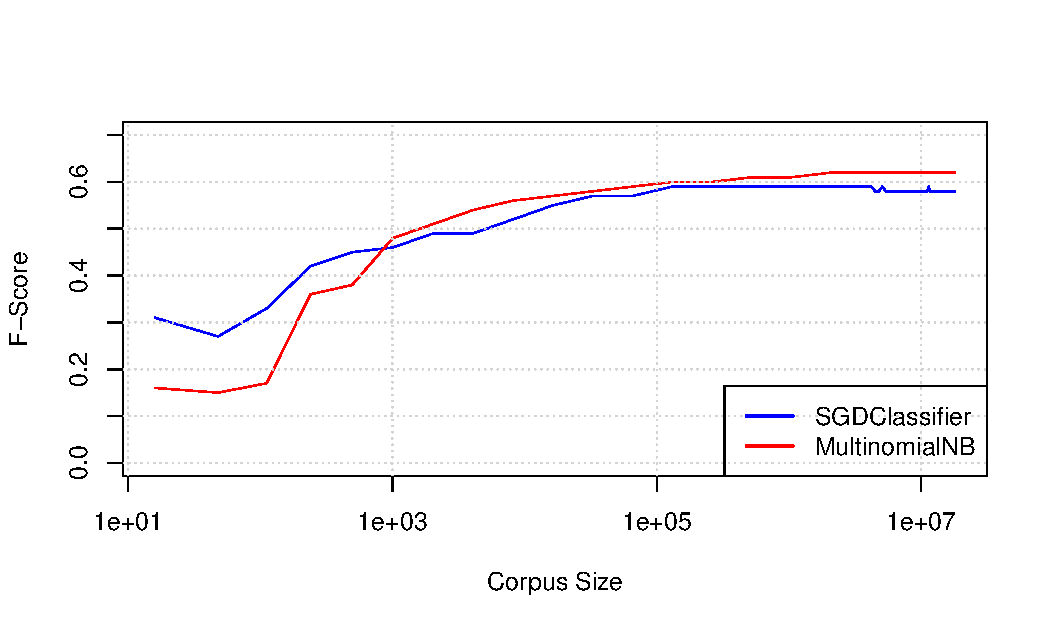
\includegraphics[scale=0.65]{minpp.pdf}
%\end{frame}
\begin{frame}{Results with full PP}
    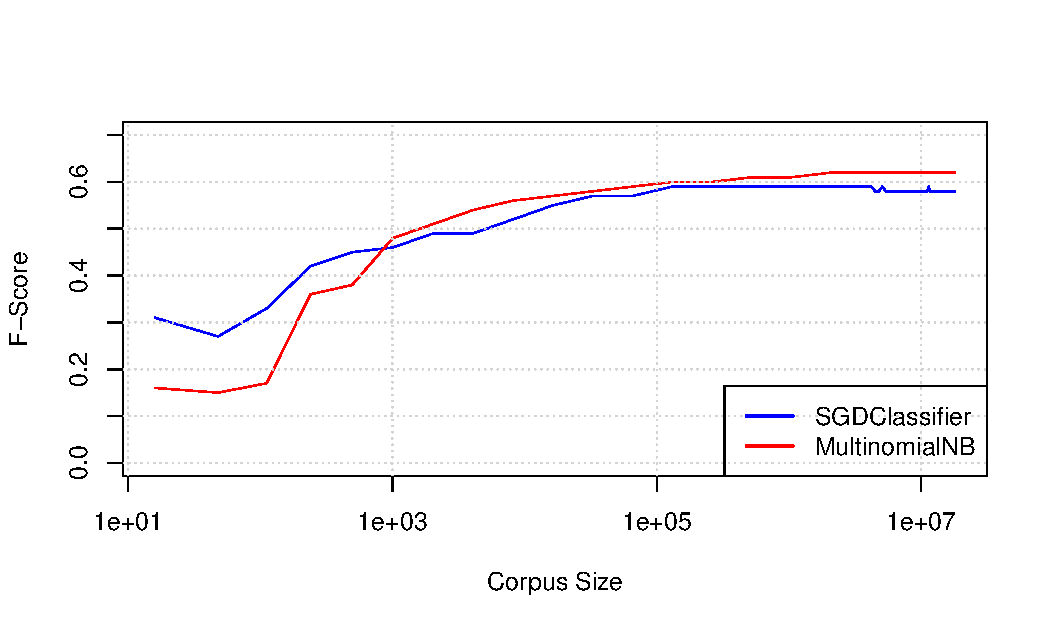
\includegraphics[scale=0.65]{fullpp.pdf}
\end{frame}

\end{document}
